\documentclass{article}
\usepackage[utf8]{inputenc}
\usepackage{subcaption}
\usepackage{amsmath}
\usepackage{amssymb}
\usepackage{hyperref}
\usepackage{titlesec}
\usepackage{xcolor}
\usepackage{fancyhdr}
\usepackage{graphicx}
\usepackage{multirow}
\usepackage[rightcaption]{sidecap}
\usepackage{verbatim}
%\usepackage{biblatex}
\usepackage [ a4paper , hmargin =1.2 in , bottom =1.5 in ] { geometry }
%\addbibresource{references.bib}
\hypersetup{
    colorlinks=true,
    linkcolor=blue,
    filecolor=magenta,      
    urlcolor=cyan,
}



% Add header and footer code here
\pagestyle{fancy}
\fancyhf{}
\fancyfoot[C]{Page \thepage}
\lhead{Transformation of R.V. and Multivariate Gaussian}
\rhead{Kavya Gupta}
%\cfoot{Page \thepage}


% You may also add path to the images optionally
\graphicspath{{./images/}}

\begin{document}

% preamble
\title{Transformation of R.V. \\ and \\ Multivariate Gaussian}
\author{Kavya Gupta}
\maketitle

% below line auto generates the table of contents
% thank me for your free 1 mark
\tableofcontents
\clearpage


%code of section 1, with lists
\section{Introduction}
In this article, we will study about the following topics of statistics:
\begin{itemize}
    \item Transformation of random variables
    \item  Multivariate Gaussian random variable 
\end{itemize}


%code of section 2, make appr
\section{Transformation of Random Variable}
Given any continuous r.v. $X$ with PDF $P_{X}(x)$ and given any function $g(X)$(defined on range of $X$) we intend to find PDF associated with the r.v. $Y=g(X)$.\\
For simplicity, let’s assume $g(.)$ is monotonic increasing.\\
Then by probability mass conservation,
%para
\[ P(a< X < b) = P(g(a)< Y < g(b) = \int_{g(a)}^{g(b)} Q(y)dy \]
%para.....
Using $y = g(x)$, we get the below relation upon simplification,
\[Q(y) = P(g^{-1}(y))\frac{dg^{-1}(y)}{dy}\]
To handle monotonically decreasing $g(.)$ as well\footnote[1]{we could have used modulus operator but I wanted things to look more complicated},
\begin{equation}
    Q(y) = \begin{cases}
        +P(g^{-1}(y))\frac{dg^{-1}(y)}{dy}, & \text{for } g(.) \text{ monotonically increasing.}\\
        -P(g^{-1}(y))\frac{dg^{-1}(y)}{dy}, & \text{for } g(.) \text{ monotonically decreasing.}
    \end{cases}
\end{equation}
For more information, refer \cite{link1}
\begin{figure}[h!]
     \centering
     \begin{subfigure}[b]{0.4\textwidth}
         \centering
         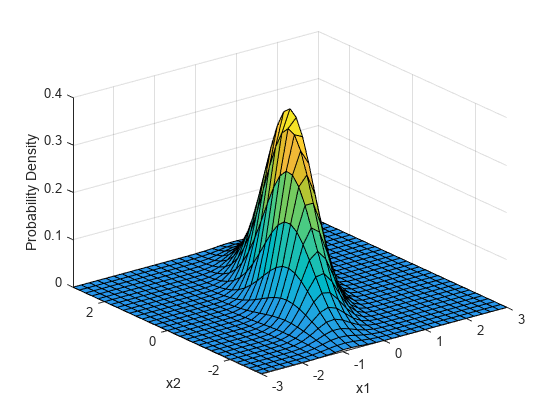
\includegraphics[width=\textwidth]{images/multivariate_gaussian.png}
         \caption{Example 1}
         \label{1a}
     \end{subfigure}
     \hfill
     \begin{subfigure}[b]{0.4\textwidth}
         \centering
         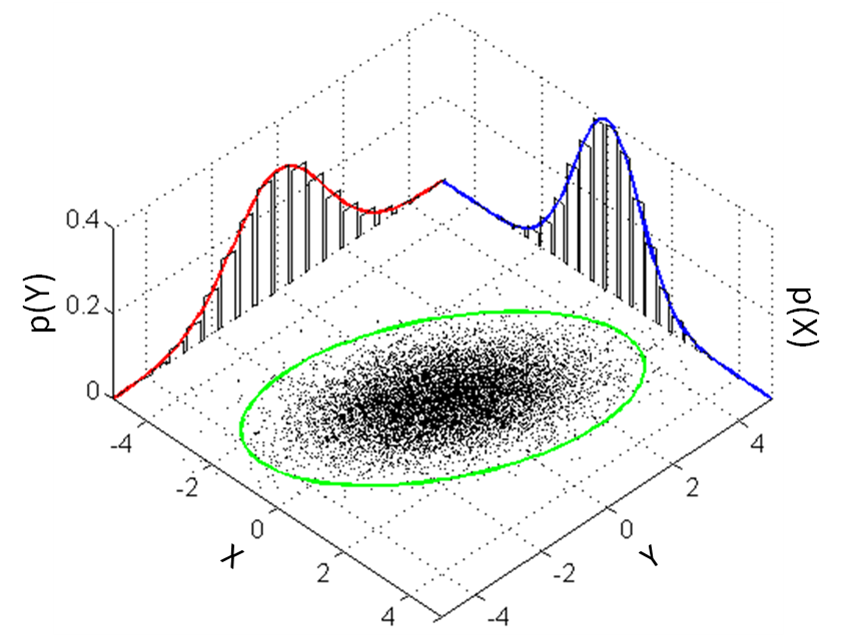
\includegraphics[width=\textwidth]{images/multivariate_normal.png}
         \caption{Example 2}
         \label{1b}
     \end{subfigure}
\end{figure}



% \begin{figure}[h!]
%     % code for subfigure, label them for using references
% \end{figure}

%code for section 3
\section{Multi-variate Gaussian Disribution}
\subsection{Definition}
Let $X$ be a vector of random variables of dimension $D$.\\
A r.v. $X$ has a joint PDF as multi-variate Gaussian distribution $\exists$ finite i.i.d. standard Gaussian \newpage r.v. $W_1, W_2, \dots W_N$ with $N > D$ such that \[ A = XW + \mu \]
Refer fig[\ref{1a}] and fig[\ref{1b}] for visual examples.This has many applications in machine learning, refer \cite{link2} and \cite{texbook}.

\subsection{A is diagonal}
In this case, the $X_i$ are independent. The standard deviation of distribution of $X_i$ is $A_{ii}$.

\subsection{A is non-singular square matrix}
Let’s take $\mu = 0$ for simplicity.\\
Similar to univariate case, where scaling was determined by $|\frac{dg^{-1}(y)}{dy}|$ the scaling for multi-variate
case is determined by determinant of matrix of derivatives, Jacobian matrix.\\
Also, $W = A^{-1}X$.We intend to find the volume of the parallelepiped formed due to this transformation.
\textbf{Claim}The volume of parallelepiped described by column vectors of matrix $A^{-1}$ is given by $det(A^{-1})$

\begin{equation}
P(X) = \frac{1}{(2\pi)^{\frac{D}{2}}}\cdot\frac{1}{\sqrt{det(C)}}\cdot exp(0.5 \cdot XT \cdot C^{-1} \cdot X)
\end{equation}

\begin{tabular}{ |p{3 cm}|p{3 cm}||p{3 cm}| }
\hline
\multicolumn{3}{|c|}{Sample Values of bivariate normal distribution}\\
\hline
x & y & f(x,y) \\
\hline
0 & 0 & 1.6\\
0 & 1 & 0.096 \\
$\sqrt{2}$ & $\sqrt{2}$ & 0.02 \\
\hline

\end{tabular}


% print the bibliography
%\printbibliography
\bibliographystyle{plain}
\bibliography{references}


\end{document}